\section{Asignación de marcos de referencia}
A continuación definiremos los pasos de \textbf{Denavit Hartenberg} para asignar marcos de referencia. Luego veremos un ejemplo.

\begin{miDefinicion}{Denavit Hartenberg - Asignación de marcos de referencia}
    Para un eslabón $i$ con dos nodos:
    \begin{enumerate}
        \item Alinear $z_i$ con el eje en movimiento de la articulación distal.
        \item Alinear $z_{i-1}$ con el eje en movimiento de la articulación proximal.
        \item La articulación distal tendrá índice $i+1$. La articulación proximal tendrá índice $i$.
        \item El origen $o$ del marco de referencia se coloca en la intersección entre el eje $z_{i}$ y el vector normal común a los ejes $z_{i-1}$ y $z_i$. 
        \item El eje $x$ se coloca sobre el vector normal anterior. Si son paralelos, $x_i$ va de $z_{i-1}$ a $z_i$. 
        \item El eje $y_i$ se elige con la regla de la mano derecha. 
    \end{enumerate}
\end{miDefinicion}

Ahora veremos un ejemplo utilizando el brazo robótico de la figura~\ref{fig:brazo-propio}. En este ejemplo, dibujaremos los ejes $z$ con lineas punteadas, esto significa que todos los ejes $z$ apuntan hacia nosotros, no apuntan a ninguna dirección dentro del dibujo en 2D. De hecho, en algunos recursos no se dibujan. 

\begin{figure}[H]
    \centering
    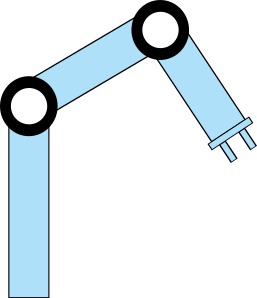
\includegraphics[width=0.35\textwidth]{imagenes/brazo-propio}
    \caption{Cadena cinemática abierta simple.}
    \label{fig:brazo-propio}
\end{figure}


\begin{itemize}
    \item Primero definimos el \textbf{marco de referencia} del mundo $(x_w, y_w, z_w)$, la letra $w$ viene de \textit{world}. El eje $y_w$ se alinea con el eslabón base (el primer eslabón) apuntando hacia el primer nodo, y el origen lo ubicamos en el inicio del eslabón base. Lo ejes $x_w$ y $z_w$ se colocan siguiendo el sistema de la mano derecha. En la figura~\ref{fig:brazo-marco-mundo} podemos ver cómo se coloca este marco.
    \begin{figure}[H]
        \centering
        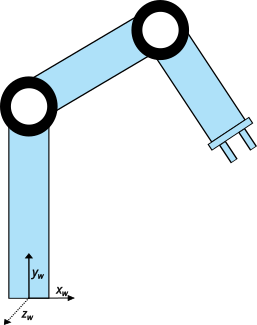
\includegraphics[width=0.35\textwidth]{imagenes/brazo-marco-mundo.png}
        \caption{Marco del mundo en cadena cinemática.}
        \label{fig:brazo-marco-mundo}
    \end{figure}
    \item Ahora procederemos a asignar un marco de referencia al primer nodo. Alineamos el eje $z_0$ con el eje en movimiento de la primera articulación. Luego alineamos el eje $x_0$ con el eslabón base, de forma que $x_0$ apunte hacia adentro del eslabón. Luego colocamos el eje $y_0$ siguiendo el sistema de la mano derecha. En la figura~\ref{fig:brazo-marco-primer-art} podemos ver cómo se asigna este marco de referencia. 
    \begin{figure}[H]
        \centering
        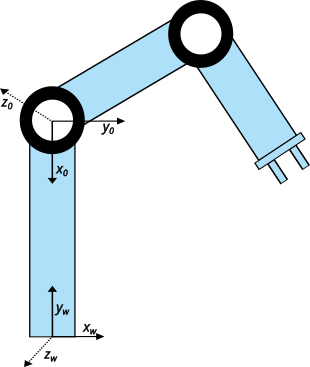
\includegraphics[width=0.35\textwidth]{imagenes/brazo-marco-primer-art}
        \caption{Marco del primer nodo.}
        \label{fig:brazo-marco-primer-art}
    \end{figure}
    \item Ahora procederemos a usar el método D-H que definimos anteriormente, pues lo definimos para eslabones con dos articulaciones. Respecto al eslabón $1$ (en este caso $i=1$), alineamos el eje $z_1$ con el eje en movimiento de la articulación distal. Alineamos el eje $z_0$ con el eje en movimiento de la articulación proximal. La articulación distal tendrá índice $2$, y la articulación proximal tendrá índice $1$. El origen $o$ del marco de referencia se coloca en la intersección entre el eje $z_1$ y el vector normal común a los ejes $z_1$ y $z_0$. El eje $x_1$ va de $z_0$ y $z_1$. El eje $y_1$ se elige con la regla de la mano derecha. La figura~\ref{fig:brazo-marco-dh} muestra cómo queda colocado este marco de referencia. 
    \begin{figure}[H]
        \centering
        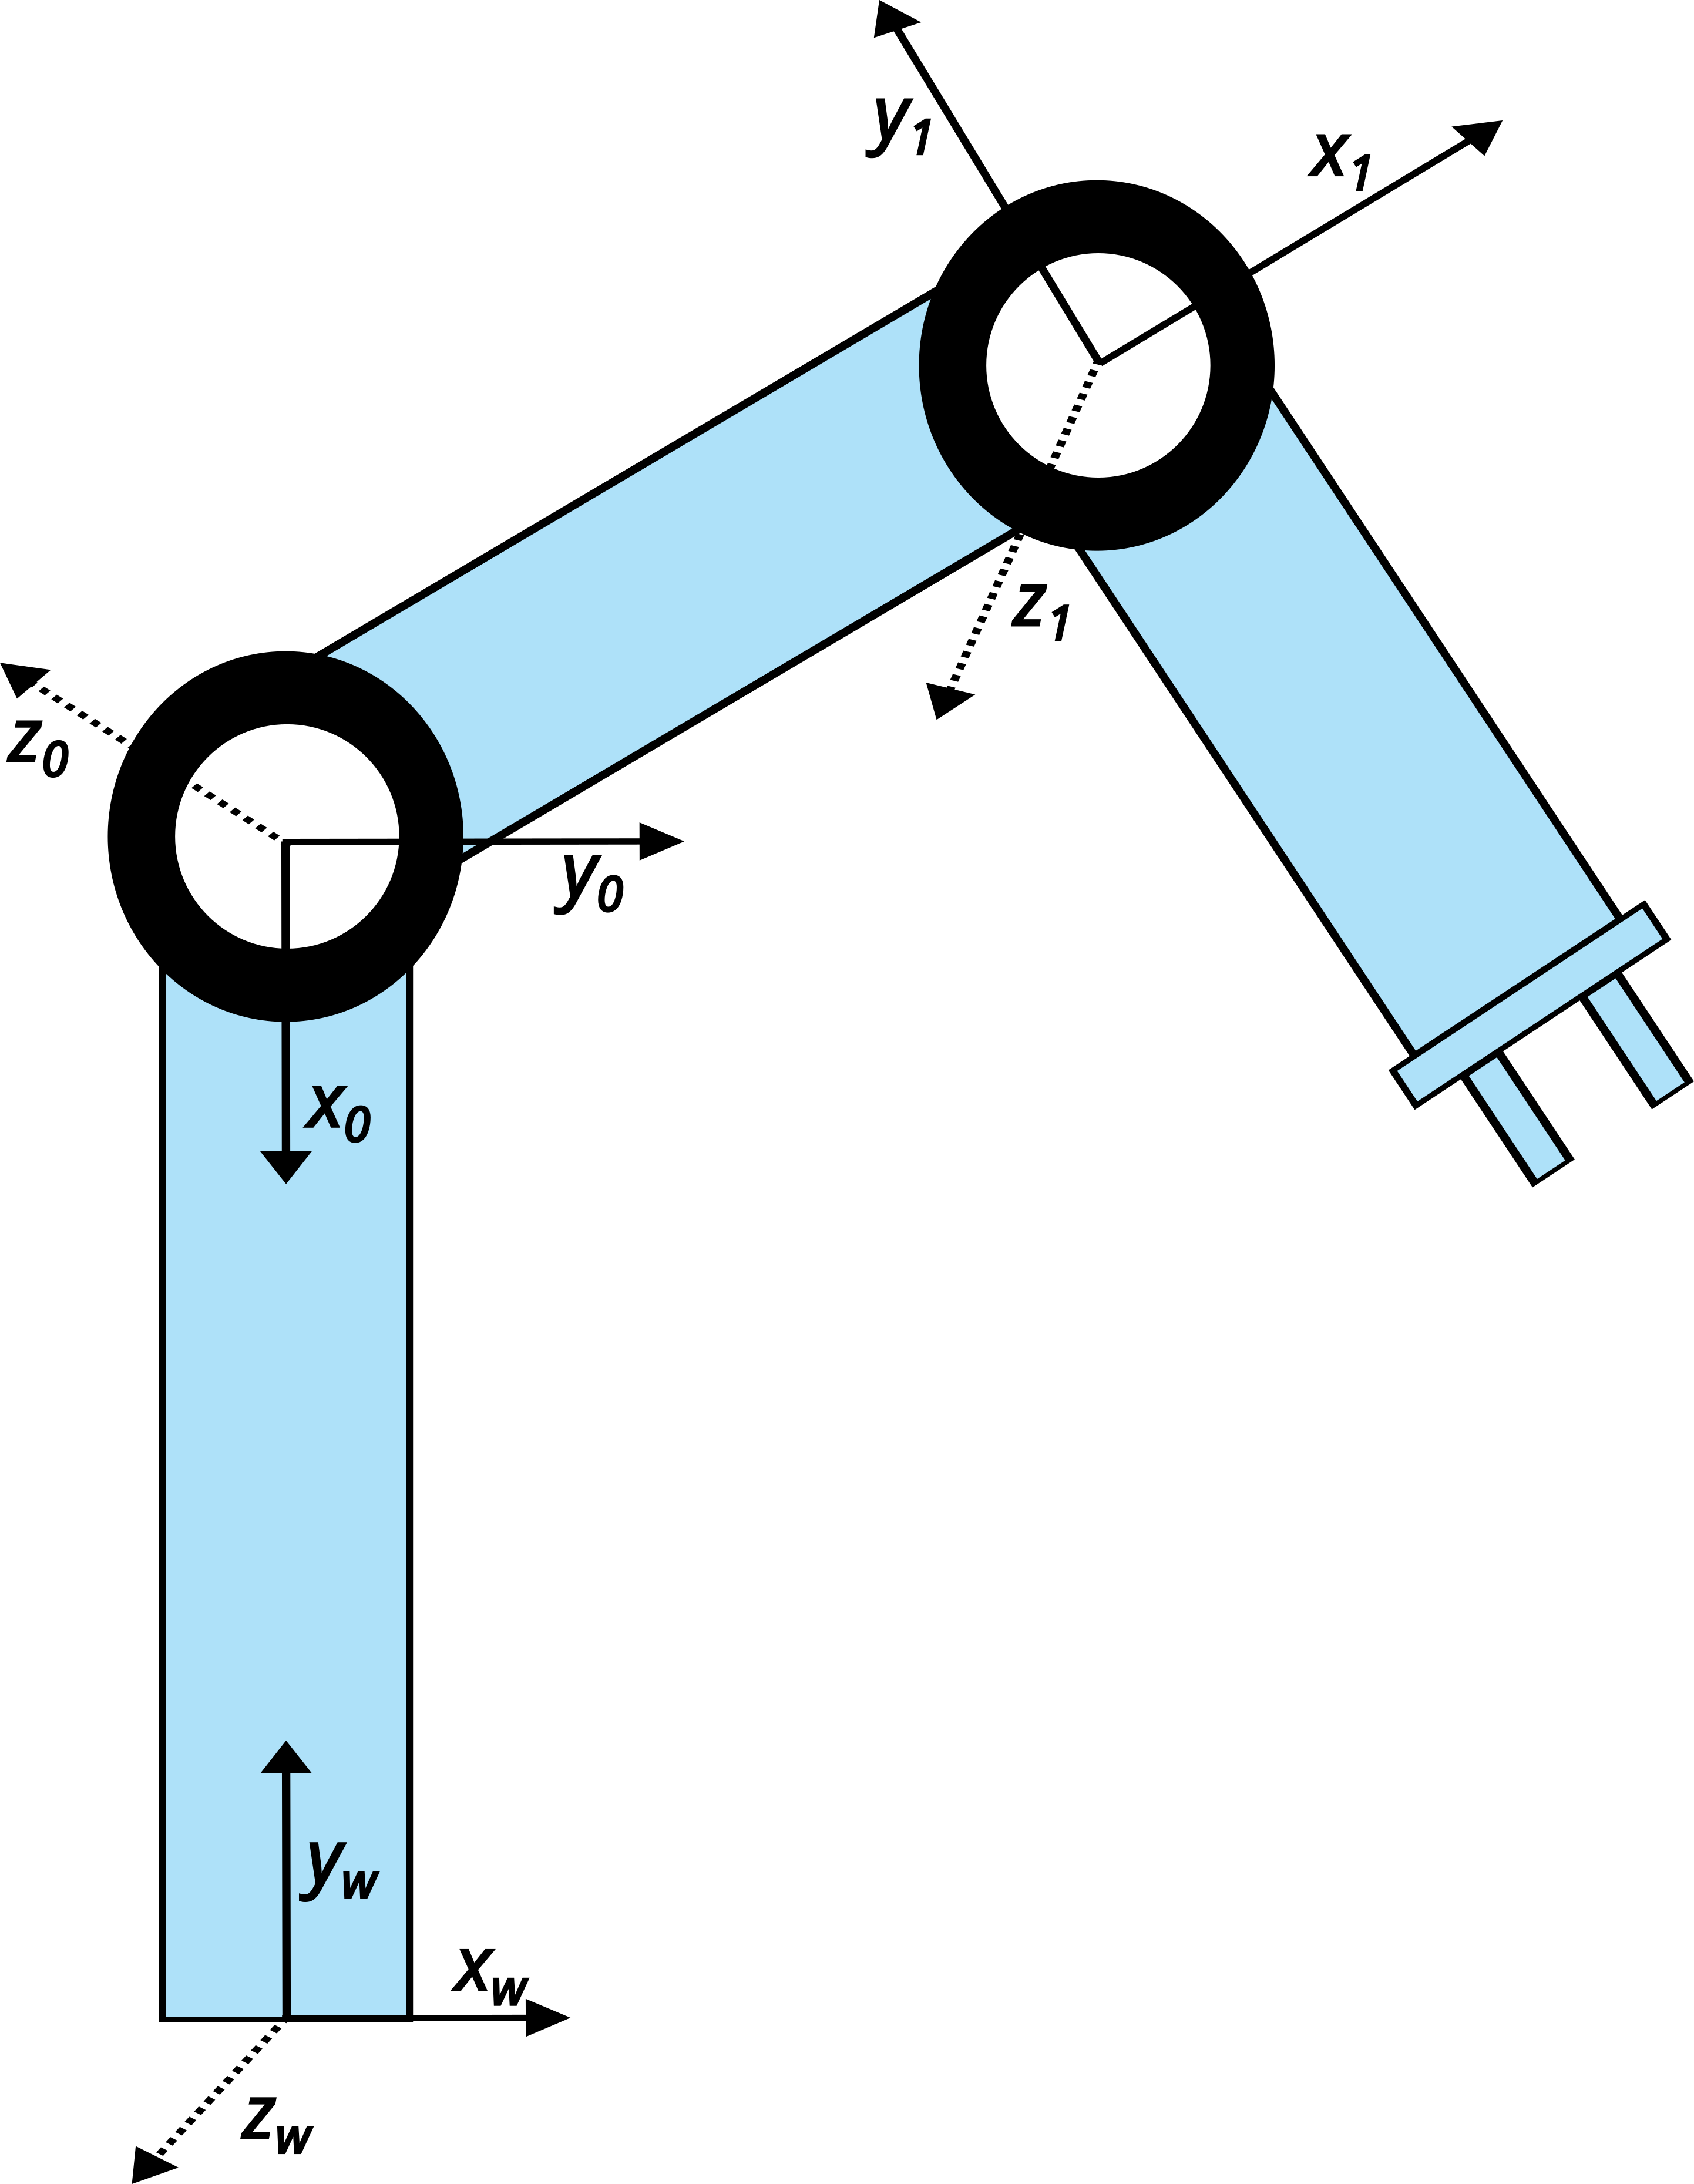
\includegraphics[width=0.35\textwidth]{imagenes/brazo-marco-dh.png}
        \caption{Marco del segundo nodo.}
        \label{fig:brazo-marco-dh}
    \end{figure}
    \item Y con eso terminamos de asinar los marcos de referencia a la cadena cinemática de la figura~\ref{fig:brazo-propio} con dos articulaciones. 
\end{itemize}